\chapter{System Design}

\section{System Architecture}

SEDS follows a four-tier containerized architecture separating presentation, application logic, message distribution, and data persistence. The Next.js frontend, Node.js/Express backend, Redis message broker, and PostgreSQL/PostGIS database each run as independent Docker containers orchestrated via Docker Compose. All inter-tier communication is strictly layered: the browser calls only the REST API, the API publishes incidents to Redis and polls/subscribes via SSE, and the API is the sole consumer of the database.

\begin{itemize}
  \item \textbf{Frontend:} Next.js 16 with React 19, MapLibre GL for WebGL map rendering, Tailwind CSS, shadcn/ui components, Zustand for state management.
  \item \textbf{Backend:} Node.js 20 + TypeScript + Express REST API; Sequelize ORM; JWT authentication; Server-Sent Events (SSE) for push notifications; Redis pub/sub for multi-responder fan-out.
  \item \textbf{Message Broker:} Redis for pub/sub fan-out of incident events to station-scoped responder channels and citizen-scoped streams; enables horizontal scaling without direct database polling.
  \item \textbf{Database:} PostgreSQL 16 with PostGIS 3.4 extension; GEOMETRY types for spatial data; GIST indexes for fast containment queries; row-level locking (SELECT FOR UPDATE) for atomic incident claims.
  \item \textbf{Infrastructure:} Docker Compose orchestrates all services; PostGIS container pre-loaded via init-postgis.sql; health checks on all services.
\end{itemize}

\section{Database Schema}

The database comprises five tables managed by Sequelize ORM with PostgreSQL 16 and PostGIS 3.4.

\begin{itemize}
  \item \textbf{users:} id, name, email, password (bcrypt), role ENUM(admin/responder/citizen), oauth\_provider ENUM(local/google/guest), verified BOOLEAN, created\_at, updated\_at.
  \item \textbf{stations:} id, name, category ENUM(POLICE/FIRE/MEDICAL), location GEOMETRY(Point, 4326), created\_at, updated\_at.
  \item \textbf{zones:} id, station\_id (FK \textrightarrow\ stations, CASCADE), boundary GEOMETRY(Polygon, 4326) with GIST index for sub-millisecond ST\_Contains containment queries.
  \item \textbf{responders:} id, user\_id (FK \textrightarrow\ users, CASCADE), station\_id (FK \textrightarrow\ stations, CASCADE), status ENUM(AVAILABLE/BUSY/OFF\_DUTY), created\_at, updated\_at.
  \item \textbf{incidents:} id, citizen\_id (FK \textrightarrow\ users), station\_id (FK \textrightarrow\ stations), responder\_id (FK \textrightarrow\ responders, nullable), category ENUM(POLICE/FIRE/MEDICAL), status ENUM(PENDING/RESPONDING/ARRIVED/RESOLVED), location GEOMETRY(Point, 4326), accepted\_at (timestamp when responder claims), created\_at, updated\_at. Incidents are claimed atomically via Postgres row-level locking (SELECT \ldots FOR UPDATE).
\end{itemize}

\section{System Flowchart and Incident Lifecycle}

\begin{figure}[H]
  \centering
  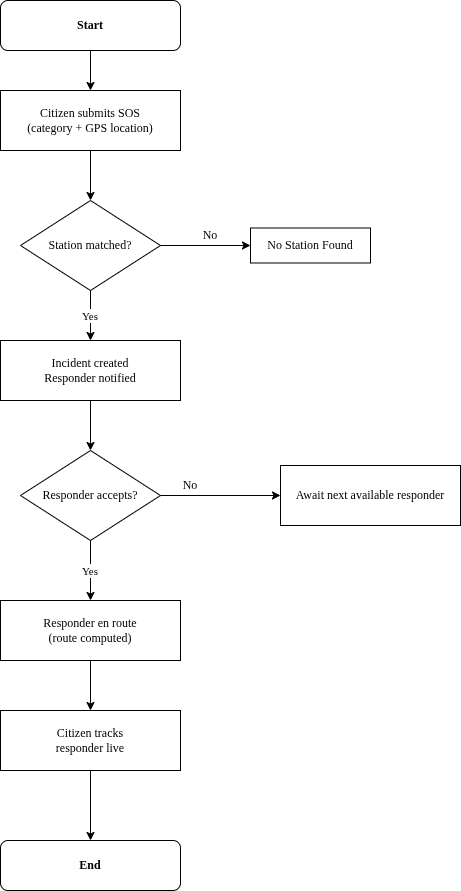
\includegraphics[width=0.7\textwidth]{Graphics/flow.png}
  \caption{System Operational Flowchart: SOS submission, zone containment / distance fallback, assignment, and responder action progression}
  \label{fig:flowchart}
\end{figure}
\FloatBarrier

The incident lifecycle follows four distinct states: \textbf{Pending} (awaiting responder claim), \textbf{Responding} (responder en route to station, or moving from station to incident location), \textbf{Arrived} (responder at scene), and \textbf{Resolved} (incident handled, responder returns to available). Each status change is atomically logged and published via Redis pub/sub to all subscribed responders at the incident's assigned station and to the originating citizen via Server-Sent Events. If SSE disconnects, clients rejoin and query the active incident endpoint to catch up within 5 seconds via polling.
